% IMPI Figure 5

\begin{figure}
\centering
\begin{tabular}{c c}
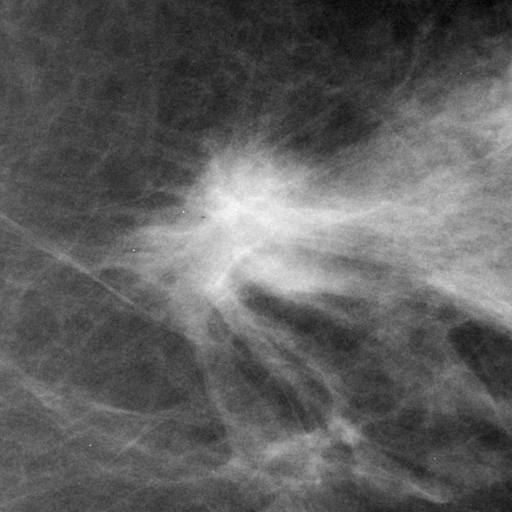
\includegraphics[width=\qtrcol]{\figpath/mammo/ipmi/mass046} &
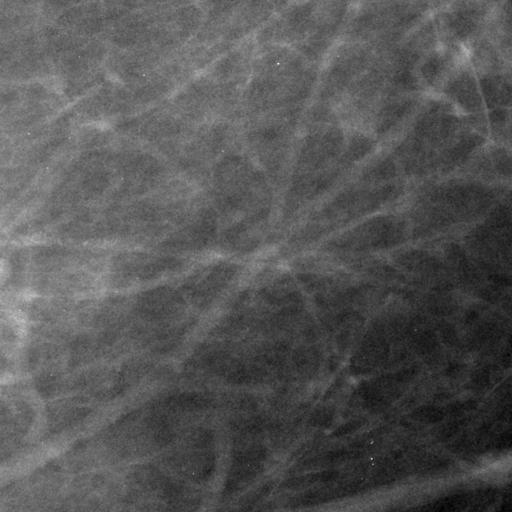
\includegraphics[width=\qtrcol]{\figpath/mammo/ipmi/norm068} \\
(a) & (b) \\
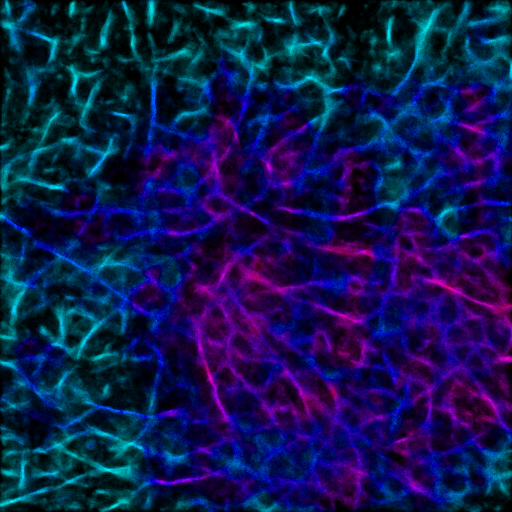
\includegraphics[width=\qtrcol]{\figpath/mammo/ipmi/spic_prob_mass046_a} &
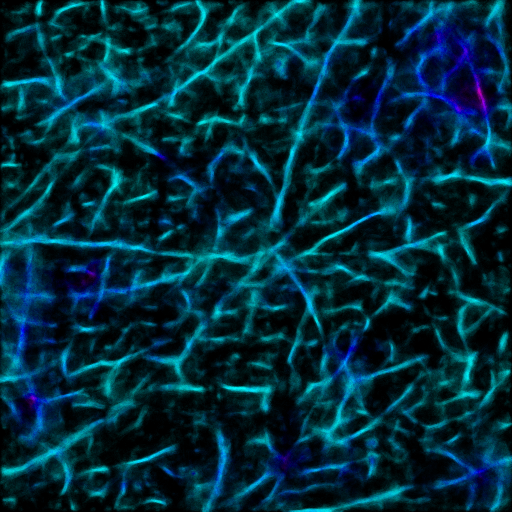
\includegraphics[width=\qtrcol]{\figpath/mammo/ipmi/spic_prob_norm068_a} \\
(c) & (d)
\end{tabular}
%
\caption{Regions depicting (a) malignant and (b) normal tissue. The corresponding spicule classification results are depicted in (c,d) using hue to indicate abnormality -- ranging from cyan (normal) to pink (spicule) -- and intensity to indicate the line detection output from the DT-CWT method.}
\label{f:mammogram_examples}
\end{figure}
